\documentclass[11pt,a4paper,oldfontcommands,oneside]{memoir}
\usepackage[utf8]{inputenc}
\usepackage{microtype}
\usepackage[dvips]{graphicx}
\usepackage{xcolor}
\usepackage{times}
\usepackage{graphicx}
\usepackage[spanish]{babel}
\usepackage[
breaklinks=true,colorlinks=true,
%linkcolor=blue,urlcolor=blue,citecolor=blue,% PDF VIEW
linkcolor=black,urlcolor=black,citecolor=black,% PRINT
bookmarks=true,bookmarksopenlevel=2]{hyperref}

\usepackage{geometry}
% PDF VIEW
% \geometry{total={210mm,297mm},
% left=25mm,right=25mm,%
% bindingoffset=0mm, top=25mm,bottom=25mm}
% PRINT
\geometry{total={210mm,297mm},
left=20mm,right=20mm,
bindingoffset=10mm, top=25mm,bottom=25mm}

\OnehalfSpacing
%\linespread{1.3}

%%% CHAPTER'S STYLE
\chapterstyle{bianchi}
%\chapterstyle{ger}
%\chapterstyle{madsen}
%\chapterstyle{ell}
%%% STYLE OF SECTIONS, SUBSECTIONS, AND SUBSUBSECTIONS
\setsecheadstyle{\Large\bfseries\sffamily\raggedright}
\setsubsecheadstyle{\large\bfseries\sffamily\raggedright}
\setsubsubsecheadstyle{\bfseries\sffamily\raggedright}


%%% STYLE OF PAGES NUMBERING
%\pagestyle{companion}\nouppercaseheads 
%\pagestyle{headings}
%\pagestyle{Ruled}
\pagestyle{plain}
\makepagestyle{plain}
\makeevenfoot{plain}{\thepage}{}{}
\makeoddfoot{plain}{}{}{\thepage}
\makeevenhead{plain}{}{}{}
\makeoddhead{plain}{}{}{}


\maxsecnumdepth{subsection} % chapters, sections, and subsections are numbered
\maxtocdepth{subsection} % chapters, sections, and subsections are in the Table of Contents


%%%---%%%---%%%---%%%---%%%---%%%---%%%---%%%---%%%---%%%---%%%---%%%---%%%

\begin{document}

%%%---%%%---%%%---%%%---%%%---%%%---%%%---%%%---%%%---%%%---%%%---%%%---%%%
%   TITLEPAGE
%
%   due to variety of titlepage schemes it is probably better to make titlepage manually
%
%%%---%%%---%%%---%%%---%%%---%%%---%%%---%%%---%%%---%%%---%%%---%%%---%%%
\thispagestyle{empty}

{%%%
\sffamily
\centering
\Large

~\vspace{\fill}

\includegraphics[scale=1]{logo.png} \\
{\huge 
\vspace{4cm}
Explicación de la Convención Denavit-Hartenberg
}
\vspace{2.5cm}

{\LARGE
Eduardo Robles Vázquez
}

\vspace{2.5cm}

Universidad Politécnica de la Zona Metropolitana de Guadalajara

\vspace{3.5cm}

Profesor: Carlos Enrique Morán Garabito

\vspace{\fill}

24 de septiembre del 2019

%%%
}%%%

\vspace{.5cm}
\hfill\break




\tableofcontents*

\clearpage

%%%---%%%---%%%---%%%---%%%---%%%---%%%---%%%---%%%---%%%---%%%---%%%---%%%
%%%---%%%---%%%---%%%---%%%---%%%---%%%---%%%---%%%---%%%---%%%---%%%---%%%

\chapter{Introducción}
Se trata de un procedimieto sistemático para describir la estructura cinemática de una cadena articulada constituida por articulaciones con un solo grado de libertad.
Para ello, a cada articulación se le asigna un Sistema de Referencia Local con origen en un punto $Qi$ y ejes ortonormales ${Xi,Yi,Zi}$, comenzando con un primer sistema de referencia fijo e inmóvil dado por los ejes ${X0,Y0,Z0}$, anclado a un punto fijo $Q0$ de la base sobre la que está montada toda la estructura de la cadena.
Este sistema de referencia no tiene por qué ser el universal con el origen en $(0,0,0)$ y la base canónica.
\vspace{2cm}
\hfill
\chapter{Asignación de Sistemas de Referencia}
Las articulaciones se numeran desde 1 hasta n. A la articulación i-ésima se le asocia su propio eje de rotación como Eje $Zi-1$, de forma que el eje de giro de la 1ª articulación es $Z0$ y el de la n-ésima articulación, $Zn-1$.
En la figura \ref{1} se muestra la estructura del Robot PUMA junto con sus articulaciones y ejes de rotación.

\begin{figure}[h]
	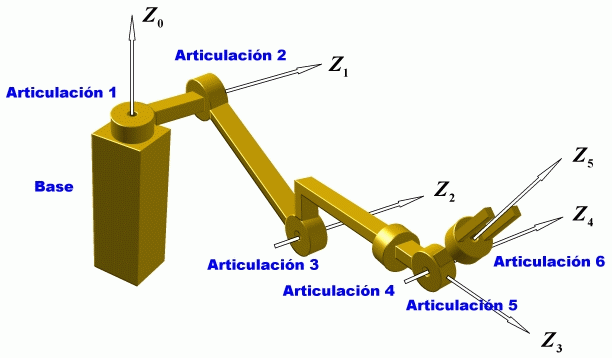
\includegraphics[scale=1]{1.png}
	\caption{Robot Puma}
	\label{1}
\end{figure}

Para la articulación i-ésima, la elección del origen de coordenadas $Qi$ y del Eje $Xi$ sigue reglas muy precisas en función de la geometría de los brazos articulados, el Eje $Yi$ por su parte, se escoge para que el sistema ${Xi, Yi, Zi}$ sea dextrógiro. La especificación de cada Eje $Xi$ depende de la relación espacial entre $Zi$ y $Zi-1$, distinguiéndose 2 casos:

\section{Zi y Z(i-1) no son paralelos}
Entonces existe una única recta perpendicular a ambos, cuya intersección con los ejes proporciona su mínima distancia. Esta distancia, $ai$, medida desde el eje $Zi-1$ hacia el eje $Zi$, es uno de los parámetros asociados a la articulación i -ésima.
La distancia di desde $Qi-1$ a la intersección de la perpendicular común entre $Zi-1$ y $Zi$ con $Zi-1$ es el segundo de los parámetros. En este caso, el eje $Xi$ es esta recta, siendo el sentido positivo el que va desde el eje $Zi-1$ al $Zi$ si $ai$ es menor que 0.
El origen de coordenadas $Qi$ es la intersección de dicha recta con el eje $Zi$.

\begin{figure}[h]
	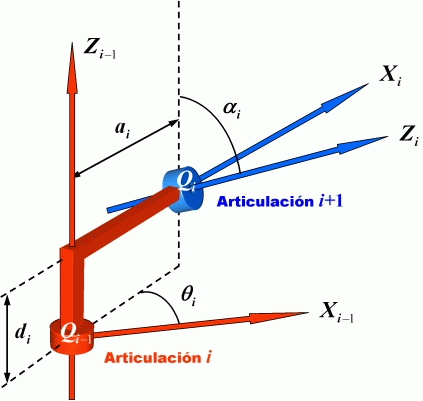
\includegraphics[scale=.75]{2.png}
	\caption{Movimiento articulaciones}
	\label{2}
\end{figure}

\section{Zi y Z(i-1) son paralelos}
En esta situación el eje $Xi$ se toma en el plano conteniendo a $Zi-1$ y $Zi$ y perpendicular a ambos. El origen $Qi$ es cualquier punto conveniente del eje $Zi$.
El parámetro $ai$ es, como antes, la distancia perpendicular entre los ejes $Zi-1$ y $Zi$, y $di$ es la distancia desde $Qi-1$.

\begin{figure}[h]
	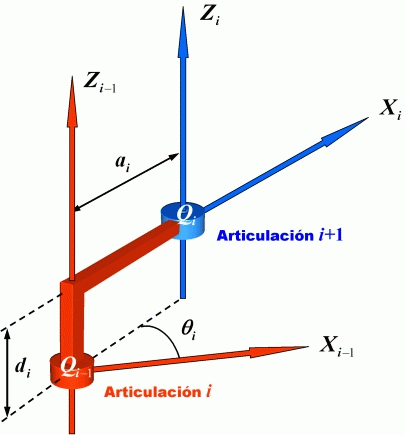
\includegraphics[scale=.75]{3.png}
	\caption{Movimiento articulaciones 2}
	\label{3}
\end{figure}

Una vez determinado el Eje $Xi$, a la articulación i -ésima se le asocia un tercer parámetro fijo ai que es el ángulo que forman los ejes $Zi-1$ y $Zi$ en relación al eje $Xi$.
Nótese que cuando el brazo i -ésimo (que une rígidamente las articulaciones $i$ e $i+1$) gira en torno al eje $Zi-1$, los parámetros $ai$, $di$, y $\alpha i$ permanecen constantes, pues dependen exclusivamente de las posiciones/orientaciones relativas entre los ejes $Zi-1$ y $Zi$, que son invariables. Por tanto, $ai$, $di$, y $\alpha i$ pueden calcularse a partir de cualquier configuración de la estructura articulada, en particular a partir de una configuración inicial estándar. Precisamente el ángulo $\theta i$ de giro que forman los ejes $Xi-1$ y $Xi$ con respecto al eje $Zi-1$ es el cuarto parámetro asociado a la articulación $i$ y el único de ellos que varía cuando el brazo $i$ gira.
Es importante observar que el conjunto de los 4 parámetros $ai$, $di$, $\alpha i$ y $\theta i$ determina totalmente el Sistema de Referencia de la articulación $i+1$ en función del Sistema de Referencia de la articulación $i$.

\vspace{2cm}
\hfill
\chapter{Transformación de Coordenadas}
De los 4 parámetros asociados a una articulación, los 3 primeros son constantes y dependen exclusivamente de la relación geométrica entre las articulaciones $i$ e $i+1$ , mientras que el cuarto parámetro $\theta i$ es la única variable de la articulación, siendo el ángulo de giro del eje $Xi-1$ alrededor del eje $Zi-1$ para llevarlo hasta $Xi$.
Sabemos que dados 2 Sistemas de Referencia:
\begin{figure}[h]
	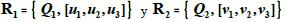
\includegraphics[scale=1]{4.png}
	\label{4}
\end{figure}\\
Con bases ortonormales asociadas, el cambio de coordenadas del segundo Sistema de Referencia al primero viene dado por:
\begin{figure}[h]
	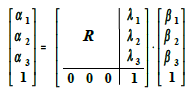
\includegraphics[scale=2]{5.png}
	\label{5}
\end{figure}\\
donde $\beta 1$, $\beta 2$, $\beta 3$ son las coordenadas de un punto en el Sistema de Referencia  $R2$ , $R$ es la matriz del Cambio de Base tal que:
\begin{figure}[h]
	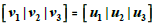
\includegraphics[scale=1.35]{6.png}
	\label{6}
\end{figure}\\
$R$ y $\lambda 1$ , $\lambda 2$, $\lambda 3$ son las coordenadas del origen del segundo Sistema de Referencia, $Q2$ respecto al primero. La expresión permite entonces obtener las coordenadas $\alpha 1$, $\alpha 2$ , $\alpha 3$ del punto en cuestión con respecto al primero de los Sistema de Referencia.
En nuestro caso, para pasar de la $(i+1)$-ésima articulación a la i -ésima, los Sistemas de Referencia son:
\begin{figure}[h]
	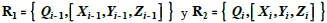
\includegraphics[scale=1.5]{7.png}
	\label{7}
\end{figure}\\
\vspace{2cm}
\hfill

\chapter{Consideraciones Finales}
La representación Denavit-Hartenberg presupone que cuando se realiza una rotación alrededor de uno de los ejes, digamos $Zi-1$, la orientación del eje $Zi$ varía debido a la acción del brazo que los une (exceptuando el caso en el que $Zi-1$ y $Zi$ son paralelos), aunque naturalmente el ángulo $\alpha i$ entre ambos ejes permanece constante.
Esta observación implica que es imposible que el eje $Zi$ tenga una orientación constante e independiente de la rotación que se efectúe alrededor de $Zi-1$, lo cual implica que la transformación de un sistema a otro no puede en ningún caso expresarse como una rotación de ángulos de Euler de $Ejes Fijos$, como la RPY.

\vspace{2cm}
\hfill
\bibliographystyle{unsrt}
\bibliography{biblio}


\end{document}

